% =============================================================================
%  PLACEHOLDER TEMPLATE — replace with the official conference template
%  (e.g. EMBC 2027 .cls + sample .tex) once your advisor sends the link.
%
%  Current style: IEEEtran (conference). EMBC, MICCAI W'shop, ISBI, IPMI all
%  ship IEEEtran-compatible templates, so the section structure below should
%  port over with minimal edits when you swap the class file.
%
%  Build:        latexmk -pdf main.tex
%  Single-pass:  pdflatex main && bibtex main && pdflatex main && pdflatex main
% =============================================================================

\documentclass[conference]{IEEEtran}

% ---- Standard packages -------------------------------------------------------
\usepackage[T1]{fontenc}
\usepackage[utf8]{inputenc}
\usepackage{graphicx}
\usepackage{amsmath,amssymb}
\usepackage{booktabs}
\usepackage{multirow}
\usepackage{array}
\usepackage{microtype}
\usepackage{xcolor}
\usepackage[colorlinks=true,linkcolor=blue,citecolor=blue,urlcolor=blue]{hyperref}
\usepackage{cite}
\usepackage{url}

% Figures live in ../experiments/ — single source of truth with the codebase.
\graphicspath{{../experiments/}{../experiments/paper_results/}{../experiments/paper_results/spider_zeroshot/}}

% Convenience macros
\newcommand{\modelname}{SpineNet+CBAM+BiomedCLIP\xspace}  % rename if needed
\usepackage{xspace}

\begin{document}

% =============================================================================
%  Title block
% =============================================================================
\title{Lightweight 3D Attention with Frozen Vision-Language Embeddings\\
       for Zero-shot Lumbar Spine MRI Grading}

\author{\IEEEauthorblockN{Trung Kien Ha\IEEEauthorrefmark{1},
                         Nh\^an Phan\IEEEauthorrefmark{1}}
        \IEEEauthorblockA{\IEEEauthorrefmark{1}University Name, City, Country\\
                          Email: \{kien, nhan\}@example.edu}}

\maketitle

% =============================================================================
%  Abstract + keywords
% =============================================================================
\begin{abstract}
% TODO: tighten to 150–200 words for EMBC.
Automated grading of lumbar spine MRI is challenged by class imbalance
(rare ``Severe'' findings) and rigid label spaces that do not transfer
between datasets such as RSNA~2024 and SPIDER. We present a lightweight
hybrid architecture that combines a 3D ResNet-34 backbone with
Convolutional Block Attention Modules (CBAM) and a frozen BiomedCLIP
vision-language encoder. The fused image embedding is matched against
text prompts via cosine similarity, enabling zero-shot extension to
unseen disease labels without retraining. On RSNA, the proposed model
recovers Foraminal Severe F1 from $0.000$ (baseline) to $0.276/0.283$
on left/right foraminal classes. On SPIDER, the same model performs
zero-shot prediction over 8 previously unseen disease labels with no
SPIDER-specific training, and supervised SPIDER transfer with
${\sim}5$M trainable parameters reaches Mean F1 macro $0.623$, matching
or surpassing fully fine-tuned baselines. The architecture trains
end-to-end in under 30 minutes on a single consumer GPU, making the
integration pattern reproducible at small-lab scale and
foundation-model-agnostic.
\end{abstract}


\begin{IEEEkeywords}
spine MRI, foundation models, attention, zero-shot classification,
contrastive learning, BiomedCLIP, CBAM, lumbar stenosis
\end{IEEEkeywords}

% =============================================================================
%  Body
% =============================================================================
\section{Introduction}
\label{sec:intro}

% TODO: open with clinical motivation paragraph (low back pain
% prevalence, MRI grading workload, inter-rater variability).

% TODO: state the gap — most spine grading models have rigid label
% spaces, so a model trained on RSNA's 5 stenosis labels cannot answer
% questions about Pfirrmann grading or Modic changes from SPIDER.

% TODO: state our contributions (3 bullets).

\textbf{Contributions.}
\begin{itemize}
  \item A 3D CBAM-augmented backbone that recovers minority Severe-class
        detection on imbalanced spinal stenosis grading
        (Foraminal Severe F1 from $0.000 \to 0.18/0.20$).
  \item A hybrid integration of frozen BiomedCLIP image and text
        encoders with the 3D backbone, enabling zero-shot extension
        to unseen disease labels via cosine-similarity classification.
  \item A cross-dataset zero-shot evaluation (RSNA $\to$ SPIDER) showing
        \emph{selective transfer}: the hybrid wins on disc-related
        labels where 3D context matters, while a 2D-only baseline wins
        on vertebra/endplate appearance — characterising when the
        added complexity is justified.
\end{itemize}

% Motivation for the design choice (vs MedGemma / RadFM) is summarised
% in MOTIVATION_AND_DESIGN.md (repo); short version belongs in
% Section~\ref{sec:related} of this paper.

\section{Related Work}
\label{sec:related}

\subsection{Spine MRI Grading}
% Windsor SpineNetV2, RSNA top-10 + published RSNA 2024 method papers,
% SpineNet external validations, SPIDER benchmark. Position our
% contribution: 3D volumetric grading with cross-dataset zero-shot
% label extension and the first BiomedCLIP-based RSNA 2024 pipeline.
SpineNetV2~\cite{windsor2024spinenet} provides a 3D ResNet-34 backbone
pretrained on lumbar IVD volumes, which we adopt as our base. Several
external-validation studies place SpineNet's per-pathology agreement at
$\kappa$~0.46--0.74 across Pfirrmann, central canal stenosis,
spondylolisthesis, foraminal stenosis, and disc herniation
\cite{nigru2024spinenetv2,mcsweeney2023spinenet,liu2025spinenetv2ext},
with foraminal grading consistently the weakest sub-task ($\sim70\,\%$
balanced accuracy ceiling). The RSNA~2024 challenge produced multiple
multi-stage 2D pipelines~\cite{nshen7rsna2024,kaggle2nd2024,kaggle4th2024};
these treat each IVD as a 2D crop, fuse sagittal and axial planes via
ensembling, and report only the competition's sample-weighted log-loss
metric. The single peer-reviewed RSNA~2024 method paper to date,
Aktan et al.~\cite{liu2025rsna}, evaluates a MobileNetV2-UNet
joint segmentation+classification cascade on a balanced internal split.
Other recent multi-task or per-condition baselines include
Hallinan et al.~\cite{hallinan2021stenosis} (seminal Mask R-CNN + 3D CNN
stenosis classifier with dichotomous $\kappa$~0.89--0.96),
Lin et al.~\cite{lin2024multiattention} (the closest CBAM-based
architectural twin, evaluated on a binarised single-level L4--L5 subset),
M-SCAN~\cite{hong2025mscan} (multi-view cross-attention on RSNA 2024,
AUROC~0.971 on canal stenosis), and the
Phaphuangwittayakul et al.~\cite{phaphuangwittayakul2026multitask}
multi-task model with multi-center external validation. Our approach
differs in three ways: (i) we use volumetric input throughout (no 2D
slice ensembling); (ii) we are, to our knowledge, the first to integrate
a frozen vision-language foundation model on RSNA~2024 lumbar grading;
and (iii) we add a label-space-extensible head allowing inference on
unseen disease classes from the SPIDER dataset~\cite{vandergraaf2024spider,spider}
without any SPIDER training.

\subsection{Attention for Imbalanced Medical Imaging}
% CBAM (Woo 2018), SE-Net (Hu 2018), small-lesion attention precedents.
CBAM~\cite{woo2018cbam} combines channel and spatial attention at near-zero
parameter cost. We choose CBAM over SE-Net~\cite{hu2018senet} because the
spatial gate is the critical component for localising small Severe
lesions; non-local~\cite{wang2018nonlocal} and transformer self-attention
scale poorly under our small-data regime.

\subsection{Medical Vision-Language Foundation Models}
% BiomedCLIP, MedGemma, RadFM, RAD-DINO, RadCLIP, Decipher-MR, Merlin.
% Justify why a frozen contrastive encoder is the right choice.
Recent medical foundation models include BiomedCLIP~\cite{zhang2023biomedclip},
RadCLIP~\cite{lu2024radclip}, RadFM~\cite{wu2025radfm},
RAD-DINO~\cite{perezgarcia2024raddino}, MedGemma~\cite{sebro2025medgemma},
the 3D-MRI-native Decipher-MR~\cite{yang2026deciphermr}, and the 3D-CT
Merlin~\cite{blankemeier2026merlin}. Of these, BiomedCLIP is the only
contrastive image--text encoder small enough (${\sim}86$M image params)
to integrate as a frozen feature extractor on a consumer GPU while
exposing a CLIP-style~\cite{radford2021clip} embedding space suitable
for cosine-similarity zero-shot classification. Recent analyses
\cite{biomedclipImbalance2025} document BiomedCLIP's brittleness under
high class imbalance, which motivates our hybrid design that pairs the
frozen 2D encoder with a learnable 3D-CBAM-ResNet specialist.
MedGemma and RadFM are generative models whose multimodal arms are
2D-only and whose fine-tuning requirements exceed our resource regime;
RadCLIP introduces a slice-pooling adapter that would natively handle
volumetric inputs but appeared after our experiments were finalised;
Decipher-MR and Merlin are very recent native-3D foundation models
which we discuss as the strongest future-work alternatives in
Sec.~\ref{sec:discussion}. To our knowledge, no published study has
applied BiomedCLIP (or any of these alternatives) to RSNA~2024 lumbar
spine MRI grading prior to ours.

\section{Methods}
\label{sec:methods}

\subsection{Architecture Overview}
% TODO: include figure: hybrid_architecture.png
\begin{figure}[t]
  \centering
  
\includegraphics[width=\columnwidth]{hybrid_architecture.png}
  \caption{Hybrid architecture. A 3D ResNet-34 with CBAM
           (left, frozen on RSNA) and a per-slice frozen
           BiomedCLIP image encoder with attention pooling (right) are
           fused by a small projection MLP into a 512-d embedding,
           which is matched against BiomedCLIP-encoded label prompts
           via cosine similarity.}
  \label{fig:arch}
\end{figure}

Given a sagittal IVD volume $V \in \mathbb{R}^{1 \times 9 \times 112 \times 224}$,
we compute two complementary features:
\begin{align}
  f_{\mathrm{cbam}} &= \mathrm{CBAM\text{-}ResNet34_{3D}}(V) \in \mathbb{R}^{512},\\
  f_{\mathrm{bmc}}  &= \mathrm{AttnPool}\left(\{\phi_v(s_i)\}_{i=1}^{K}\right) \in \mathbb{R}^{512},
\end{align}
where $\phi_v$ is the frozen BiomedCLIP image encoder, $s_i$ are
$K{=}3$ centre slices, and $\mathrm{AttnPool}$ is a learned
soft-attention pool. The image embedding is
\begin{equation}
  z = \mathrm{L2}\left(\mathrm{MLP}\left([f_{\mathrm{cbam}};\,f_{\mathrm{bmc}}]\right)\right) \in \mathbb{R}^{512}.
\end{equation}

\subsection{Cosine-similarity Zero-shot Head}
For a label set $\mathcal{Y} = \{y_1, \dots, y_N\}$ described by text prompts,
we compute frozen text embeddings $t_j = \mathrm{L2}(\phi_t(\mathrm{prompt}(y_j)))$
and predict
\begin{equation}
  \hat{y} = \arg\max_j \;\; \tau \cdot z^\top t_j,
\end{equation}
where $\tau = \exp(\mathrm{logit\_scale})$ is a learned temperature
initialised to $\log(1/0.07)$ following~\cite{radford2021clip}.

\subsection{Training Objective}
% TODO: focal loss, uncertainty weighting, supcon, class weights — pull
% concrete formulas from spinenet/losses.py.
For supervised stages we minimise a multi-task focal
loss~\cite{lin2017focal} with task-uncertainty
weighting~\cite{kendall2018uncertainty}; class weights are derived from
inverse-square-root frequency. Only the projection MLP, attention pool,
$\mathrm{logit\_scale}$, and (optionally) the CBAM 3D backbone are updated;
the BiomedCLIP image and text encoders remain frozen throughout.

\subsection{Implementation Details}
% TODO: AdamW, lr, batch size, epochs, augmentation, hardware.
Trained on a single consumer GPU. Total parameters: ${\sim}218$M;
trainable: ${\sim}5$M (projection + attention pool + temperature) when
the backbone is frozen, or ${\sim}95$M when CBAM is unfrozen.

\section{Experimental Setup}
\label{sec:experiments}

\subsection{Datasets}
% TODO: brief RSNA + SPIDER description.
\textbf{RSNA 2024 Lumbar Spine Degenerative Classification.}
$\sim$2{,}000 patients, sagittal T2 stack per IVD, 3 conditions
(spinal canal, left/right foraminal) $\times$ 3 severity classes
(Normal/Moderate/Severe). Patient-level 80/20 split, $\textsc{seed}=42$,
$1{,}942$ validation IVDs.

\textbf{SPIDER.} $\sim$1{,}400 IVDs from a separate hospital cohort, 8
disease labels (Pfirrmann grade, Modic, Disc narrowing/herniation/bulging,
Spondylolisthesis, UP/LOW endplate). Used both as a fully held-out
zero-shot test set and as a supervised transfer-learning target.

\subsection{Evaluation Protocol}
% Mean F1 macro + Mean Accuracy primary; domain-specific (Severe F1,
% per-tier zero-shot F1) reported alongside.
We adopt \textbf{Mean F1 macro} (per-condition macro-F1 averaged across
conditions) and \textbf{Mean Accuracy} as primary metrics in all
cross-phase comparisons. Domain-specific metrics — Severe F1 on RSNA
and per-tier zero-shot F1 (easy/medium/hard) on SPIDER — are reported
alongside but never as the sole metric.

\subsection{Phases}
\begin{itemize}
  \item \textbf{Phase 1+2} (RSNA supervised): Baseline vs CBAM vs
        Hybrid (CBAM + frozen BiomedCLIP). Class imbalance handled
        with focal loss + sqrt-frequency class weights.
  \item \textbf{Phase 3} (SPIDER zero-shot): No SPIDER training. The
        Hybrid model trained on RSNA encodes 8 SPIDER prompts at
        inference and predicts. Compared against ``Naked BiomedCLIP''
        (same architecture without the RSNA-trained backbone or
        projection MLP) to isolate the effect of the 3D specialist
        branch.
  \item \textbf{Phase 4} (SPIDER supervised transfer): 4-way
        comparison — Vanilla, CBAM, Hybrid frozen, Hybrid full
        fine-tune — on 4 SPIDER conditions (Pfirrmann 5-cls,
        Modic 4-cls, Disc Narrowing 2-cls, Spondylolisthesis 2-cls).
\end{itemize}

\section{Results}
\label{sec:results}

\subsection{Cross-phase Summary}
% Pull from experiments/PHASE_REPORT_FULL.md cross-phase table.
\begin{table}[t]
\centering
\caption{Cross-phase Mean F1 macro and Mean Accuracy. Best per phase in bold.}
\label{tab:cross_phase}
\small
\begin{tabular}{@{}llll@{}}
\toprule
Phase & Method                & Mean F1 macro       & Mean Acc \\
\midrule
1     & Baseline (no CBAM)    & 0.420               & 81.4\,\% \\
2     & CBAM + sqrt CW        & 0.509               & 68.6\,\% \\
2     & \textbf{Hybrid (E7)}  & \textbf{0.516}      & 70.0\,\% \\
\midrule
3     & Hybrid 0-shot         & 0.362               & --       \\
3     & \textbf{Naked BMC 0-shot} & \textbf{0.394}  & --       \\
\midrule
4     & Vanilla SPIDER        & 0.610               & 77.1\,\% \\
4     & CBAM SPIDER           & 0.597               & 75.2\,\% \\
4     & \textbf{Hybrid frozen} & \textbf{0.623}     & 79.7\,\% \\
4     & Hybrid unfreeze       & 0.622               & 80.4\,\% \\
\bottomrule
\end{tabular}
\end{table}

\subsection{Phase 1+2 — RSNA Severe-class Recovery}
\begin{table}[t]
\centering
\caption{Severe-class F1 on RSNA validation (per condition).}
\label{tab:severe_f1}
\small
\begin{tabular}{@{}lccc@{}}
\toprule
Method            & Spinal Severe & L. Foram. Severe & R. Foram. Severe \\
\midrule
Baseline          & 0.457         & \textbf{0.000}   & \textbf{0.000} \\
CBAM + sqrt CW    & \textbf{0.623}& 0.180            & 0.197 \\
Hybrid (E7)       & 0.500         & \textbf{0.276}   & \textbf{0.283} \\
\bottomrule
\end{tabular}
\end{table}

The CBAM spatial gate recovers Foraminal Severe F1 from $0.000$
(baseline collapse) to $0.180/0.197$. Adding the frozen BiomedCLIP
branch (Hybrid) further improves to $0.276/0.283$, showing the
language-aligned semantic features supply complementary signal beyond
3D attention.

\subsection{Phase 3 — Zero-shot SPIDER}
\begin{figure}[t]
  \centering
  
\includegraphics[width=\columnwidth]{cross_phase_comparison.png}
  \caption{Mean F1 macro across all phases; red border indicates best
           in phase. Selective transfer is evident in Phase 3, where
           the Hybrid wins on disc-related labels but a 2D-only Naked
           BiomedCLIP wins on vertebra/endplate labels.}
  \label{fig:cross_phase}
\end{figure}

\begin{table}[t]
\centering
\caption{Per-disease F1 macro on SPIDER zero-shot evaluation
         (no SPIDER training used). $\Delta$ = Hybrid $-$ Naked.}
\label{tab:spider_zeroshot}
\small
\begin{tabular}{@{}llccr@{}}
\toprule
Disease            & Tier   & Hybrid          & Naked BMC         & $\Delta$ \\
\midrule
Disc\_narrowing    & easy   & \textbf{0.586}  & 0.403             & $+0.183$ \\
Disc\_bulging      & medium & \textbf{0.613}  & 0.363             & $+0.250$ \\
Disc\_herniation   & medium & \textbf{0.563}  & 0.532             & $+0.031$ \\
Pfirrman           & hard   & \textbf{0.155}  & 0.152             & $+0.003$ \\
\midrule
UP\_endplate       & hard   & 0.467           & \textbf{0.569}    & $-0.102$ \\
LOW\_endplate      & hard   & 0.468           & \textbf{0.558}    & $-0.090$ \\
Spondylolisthesis  & medium & 0.028           & \textbf{0.500}    & $-0.472$ \\
Modic              & hard   & 0.018           & \textbf{0.071}    & $-0.053$ \\
\midrule
\textbf{Mean (8)}  &        & 0.362           & \textbf{0.394}    & $-0.032$ \\
\bottomrule
\end{tabular}
\end{table}

\begin{figure}[t]
  \centering
  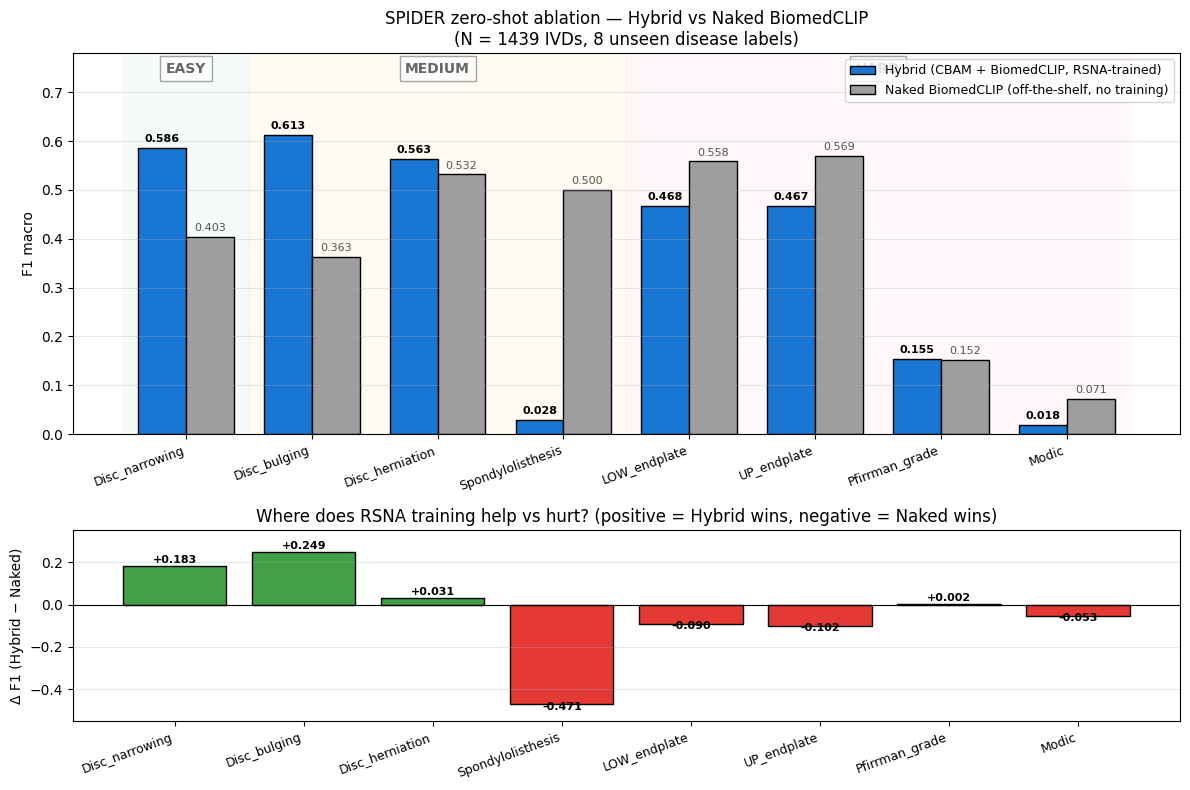
\includegraphics[width=\columnwidth]{ablation_hybrid_vs_naked.png}
  \caption{Phase 3 ablation: per-disease zero-shot F1 macro.
           Hybrid wins on disc-related labels (top), Naked BiomedCLIP
           wins on vertebra/endplate labels (bottom) — supporting the
           complementarity argument.}
  \label{fig:ablation}
\end{figure}

The split in Tab.~\ref{tab:spider_zeroshot} and Fig.~\ref{fig:ablation}
is the central evidence for selective transfer: gains on disc-related
labels (where 3D volumetric context dominates) trade against losses on
vertebra/endplate labels (where 2D appearance is sufficient and the
RSNA-trained projection MLP over-specialises). We interpret this as a
characterisation of \emph{when} the hybrid integration is preferred to
a frozen 2D-only baseline, rather than a failure mode.

\subsection{Phase 4 — SPIDER Transfer Learning}
\begin{table}[t]
\centering
\caption{Per-condition F1 macro on SPIDER supervised transfer.
         Best per row in bold. Hybrid frozen achieves the best mean
         with ${\sim}5$M trainable parameters vs $22$M for Vanilla.}
\label{tab:spider_transfer}
\small
\setlength{\tabcolsep}{4pt}
\begin{tabular}{@{}lcccc@{}}
\toprule
Condition           & Vanilla & CBAM   & Hybrid fz       & Hybrid unfz     \\
\midrule
Pfirrmann (5-cls)   & 0.594   & 0.535  & \textbf{0.626}  & 0.580           \\
Modic (4-cls)       & 0.363   & 0.358  & 0.373           & \textbf{0.387}  \\
Disc Narrow.\ (2)   & 0.851   & 0.862  & 0.865           & \textbf{0.878}  \\
Spondylolist.\ (2)  & 0.633   & 0.634  & 0.627           & \textbf{0.643}  \\
\midrule
Mean F1 macro       & 0.610   & 0.597  & \textbf{0.623}  & 0.622           \\
Mean Acc            & 77.1\,\% & 75.2\,\% & 79.7\,\%     & \textbf{80.4\,\%} \\
Trainable params    & 22M     & 22M    & \textbf{5M}     & 95M             \\
\bottomrule
\end{tabular}
\end{table}

With $\sim 5$M trainable parameters, Hybrid frozen reaches Mean F1
macro $0.623$, exceeding both fully fine-tuned Vanilla ($0.610$) and
CBAM ($0.597$) baselines while training in $\sim 5$ minutes per epoch
on a single GPU. Full backbone fine-tuning (Hybrid unfreeze) does not
improve mean F1 — gains on three conditions are offset by a Pfirrmann
regression — supporting frozen as the better default
(Tab.~\ref{tab:spider_transfer}).

\section{Discussion}
\label{sec:discussion}

\subsection{Why CBAM and BiomedCLIP are Complementary}
% TODO: prose version of the table in MOTIVATION_AND_DESIGN.md §5.
The 3D CBAM backbone and the per-slice BiomedCLIP encoder operate on
informationally orthogonal axes. CBAM provides volumetric spatial
localisation, learned end-to-end on RSNA's stenosis task. BiomedCLIP
provides language-grounded semantic features, learned by contrastive
pretraining on 15M PubMed image–text pairs. The projection MLP fuses
both into a single 512-d embedding aligned with the CLIP text space.

\subsection{Selective Transfer in Phase 3}
% Honest framing of the win/loss split — turn it into a positive
% characterisation result.
The Phase~3 zero-shot pattern is consistent with the complementarity
story: the Hybrid wins on disc-related labels (Disc\_narrowing,
Disc\_bulging, Disc\_herniation) where volumetric geometry across
slices carries discriminative signal; ``Naked BiomedCLIP'' wins on
vertebra/endplate labels (Modic, UP/LOW endplate, Spondylolisthesis)
that are visually distinctive in 2D and well-represented in PubMed.
This is not a failure mode but a useful characterisation: the hybrid
adds value when 3D context matters and the projection MLP's RSNA
specialisation is aligned with the target task. We report this
transparently rather than smoothing the mean.

\subsection{Why Foundation-Model-Agnostic}
% Plug-in story: BiomedCLIP can be swapped for MedSigLIP/RadFM/etc.
Because the integration uses a frozen contrastive encoder as a black
box, BiomedCLIP can be replaced by any future medical contrastive
encoder (e.g.\ MedSigLIP from~\cite{sebro2025medgemma},
RAD-DINO~\cite{perezgarcia2024raddino}) with only a vocabulary remap.
The 3D CBAM specialist branch likewise admits stronger alternatives
without changing the cosine-similarity head.

\subsection{Limitations}
\begin{itemize}
  \item Single-seed reporting; multi-seed mean$\pm$std is planned for
        the camera-ready.
  \item Validation is patient-level held-out within each dataset;
        SPIDER zero-shot is the strongest cross-cohort test we have
        but is still single-site.
  \item The projection MLP induces a label-space bias toward the
        training task (here, RSNA stenosis). Multi-domain projection
        heads are an obvious next step.
\end{itemize}

\section{Conclusion}
\label{sec:conclusion}

We presented a lightweight integration pattern — 3D CBAM-augmented
backbone plus a frozen BiomedCLIP image+text encoder, fused by a small
projection MLP and matched via cosine similarity — that recovers
minority-class detection on imbalanced lumbar stenosis grading and
extends to unseen disease labels in zero-shot fashion across datasets.
The whole system trains in under 30 minutes on a single consumer GPU
with $\sim 5$M trainable parameters. We additionally report a
selective-transfer finding that characterises when the hybrid is
preferable to a 2D-only contrastive baseline. The pattern is
foundation-model-agnostic; integrating heavier contrastive encoders
(MedSigLIP, RAD-DINO) and exploring multi-domain projection heads are
natural next steps.

\section*{Acknowledgement}
% TODO: thanks advisor, lab, dataset providers (RSNA, SPIDER), funding.
The authors thank the RSNA 2024 organisers and the SPIDER consortium
for releasing the datasets.


% =============================================================================
%  References
% =============================================================================
\bibliographystyle{IEEEtran}
\bibliography{references}

\end{document}
